
\documentclass{article}

%encoding
%--------------------------------------
\usepackage[utf8]{inputenc}
\usepackage[T1]{fontenc}
%--------------------------------------

\usepackage{geometry}
\usepackage{amsmath}
\usepackage{graphicx}
\usepackage{float}

\usepackage[brazilian]{babel}
\usepackage{hyphenat}
\hyphenation{mate-mática recu-perar}

 \geometry{
 a4paper,
 total={170mm,257mm},
 left=20mm,
 top=20mm,
 }

\title{Relatório do trabalho 2}
\date{17/04/2019}
\author{Allan Nozomu Fukasawa RA:163527}

\begin{document}
\maketitle

\section{Introdução}

O objetivo deste trabalho é implementar técnicas de pontilhado (half-toning) para alterar um imagem em níveis de cinza para uma em duas cores. "As técnicas de pontilhado visam reduzir a quantidade de cores (quantização de cores) utilizadas para exibir
uma imagem, procurando manter uma boa percepção por parte do usuário". \cite{Helio:1}

Serão utilizados tanto a técnica de pontilahdo ordenado  utilizando duas máscaras quanto a pontilhada com difusão de erro por Floyd-Steinberg. 

\section{Componentes}

Está sendo enviado junto a este relatório, o arquivo Trabalho 2.ipynb onde contém todo o código executado durante este trabalho, imagens utilizadas no processamente, uma pasta de resultados e a especificação do trabalho.

Foram utilizadas duas imagens bem distintas para comparar os resultados obtidos no processamento delas. A baboon.pgm (Figura \ref{Fig:baboon1}) que apresenta um grande número de detalhes e poucas regiões uniformes e a sonnet.pgm (Figura \ref{Fig:soneto1}) uma imagem bem simples um texto borrado e com diferentes graus de sombreamento.

\subsection{O Programa}

O programa foi implementado com Jupyter Notebooks, usando Python 3.7.1. As bibliotecas utilizadas no desenvolvimento do programa foram, com suas respectivas versões: 

\begin{itemize}
    \item numpy (1.15.4): para manipulação dos vetores.

    \item matplotlib (3.0.2): visualização dos dados, resultados finais e intermediários.

    \item opencv (3.4.2): realização da leitura e escrita das imagens, transformação das cores e normalização dos dados. Em especial, deve ser utilizada a versão 3.4.2 pois as anteriores não permitem salvar em formato pbm.
\end{itemize}

\subsection{Formato das imagens}

As imagens de entrada estão no formato .pgm, tanto no formato binário quanto no formato ASCII. Já as imagens de saída estão no formato .pbm, específico para imagens monocromáticas. Todas as imagens resultantes se encontram na pasta results.

\section{Solução}

\subsection{Leitura das imagens}

A imagem de entrada é lida com função \textbf{cv2.imread} que armazena a imagem em um \textbf{numpy.ndarray} de 3 dimensões (MxNx3).

Depois de lida, a imagem é convertida para níveis de cinza pela função \textbf{cv2.cvtColor} e também tem seus valores convertidos para float para facilitar na normalização e também para suportar somas que extrapolam os limites. Dessa forma, não é necessário se preocupar com overflow e underflow dos números nas operações.

\subsection{Escrita das imagens}

Também foi feito uma função auxiliar para facilitar na saída das imagens. Não é necessário normalizar a imagem uma vez que ela já se encontra monocromática após os processos realizados. A escrita da imagem é feita utilizando a função \textbf{cv2.imwrite} 

\subsection{Plotagem das imagens}

Foi utilizado para visualização dos resultados as funções de plotagem de imagens em \textbf{matplotlib.pyplot}, utilizando a paleta de cores em escalas de cinza. Não foi necessário fazer a normalização para a visualização dos dados, porque a função já realiza uma normalização linear.

\subsection{Pontilhado ordenado}

O algoritmo de pontilhado ordenado utiliza um conjunto de padrões pré-definidos, em formatos de matrix, formados por pontos pretos e brancos. Os valores das células da matriz foram utilizados como limiares, e para cada pixel normalizado, é substituído por preto se o número for menor que o valor correspondente da matriz, senão, por branco. Foram utilziados neste trabalho, duas matrizes de pontilhado ordenado, uma de tamanho $ M_{3x3} $ e uma mais conhecida (Bayer) de tamanho $ M_{4x4} $

Note que ao fazer esta operação, estamos increscentando o número de pixels da imagem pelo número de valores contidos nas máscaras. Portanto, as novas imagens após o processamento com a matrix $ M_{3x3} $ terão suas alturas e larguras triplicados. Similar ocorre com a matrix de Bayer $ M_{4x4} $ onde suas dimensões são multiplicadas por 4. 

Para realizar tal função foi utilizado operações de matriz do numpy. Primeiramente foi extendido as dimensões da imagem utilizando \textbf{numpy.reshape} para comportar, ao invés somente  o pixel, matrizes do tamanho da máscara. Logo uma imagem inicial $ I_{MxN} $ passará a ser $ I_{MxNxLxL} $ sendo L o tamanho da máscara aplicada. Depois foi feito um filtro simples em cada um desses matrizes dentro de cada elemento que antes era um pixel. Por fim, foi feito algumas operações para retornar a imagem nova de $ I_{MxNxLxL} $ para $ I_{MLxNL} $, imagem de dimensões multiplicadas por L. Para isso foi utilizado \textbf{numpy.hstack} duas vezes.

\subsubsection{Matrix de pontilhado ordenado $ M_{3x3} $}

A primeira matrix de pontilhado ordenado foi a seguinte matrix quadrada de tamanho 3:

\begin{center}
$
M_{3x3} = \begin{array}{|c|c|c|}
  \hline
  6 & 8 & 4 \\ 
  \hline
  1 & 0 & 3 \\ 
  \hline
  5 & 2 & 7 \\ 
  \hline
 \end{array}
$
\end{center}

O que acarretou em 10 padrões diferentes de tons monocromáticos. Os resultados obtidos foram as Figuras \ref{Fig:baboon2} e \ref{Fig:soneto2}.

\begin{figure}[h!]
    \centering
    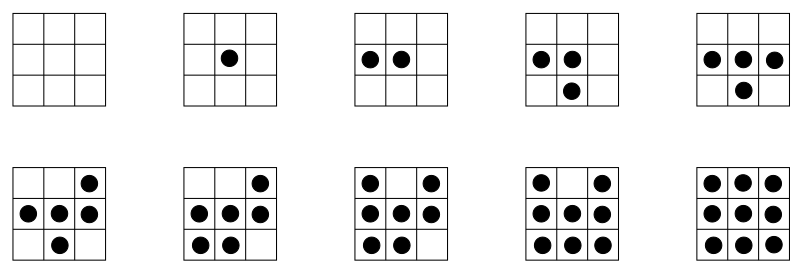
\includegraphics[width=0.7\linewidth]{padroes.png}
    \caption{Dez padrões de $3X3$ pixels}
    \label{fig:original}
\end{figure}

\subsubsection{Matrix de pontilhado ordenado Bayer}

A segunda matrix de pontilhado ordenado foi a conhecida matrix de pontilhado ordenado de Bayer, que segue a seguinte configuração:

\begin{center}
$
M_{4x4} = \begin{array}{|c|c|c|c|}
  \hline
  0 & 12 & 3 & 15 \\ 
  \hline
  8 & 4 & 11 & 7 \\  
  \hline
  2 & 14 & 1 & 13 \\ 
  \hline
  10 & 6 & 9 & 5 \\ 
  \hline
 \end{array}
$
\end{center}

Ela possui 17 diferentes padrões de $4x4$ pixels. Seguindo a mesma lógica de atribuição da matriz anterior. Os resultados obtidos foram as Figuras \ref{Fig:baboon3} e \ref{Fig:soneto3}.

\subsubsection{Comparação dos pontilhados ordenados}

Entre os filtros do baboon.pgm, não apresentou grandes diferenças uma vez que o nível de detalhamento nas duas imagens está bem alta e é possível obter uma boa persepção da imagem.

Porém, se tratando da sonnet.pgm, algumas diferenças puderam ser notadas referentes a quantidade de níveis de sombreamento presente nas duas imagens. A matrix de pontilhado ordenado $ M_{3x3} $ apresentou um número inferior a quantidade de sombras na matrix de Bayer. Isso se deve a maior quantidade de distribuição normalizada. Enquanto que na matrix $ M_{3x3} $ apresenta apenas 10 possibilidades, a de Bayer possui 17. Também em ambas, não é possível ler o texto inteiro de forma clara na imagem. Isso piora conforme o fundo vai ficando mais escuro se aproximando do brilho das letras.

\subsection{Algoritmo de Floyd-Steinberg}

O algoritmo de Floyd-Steinberg também tranforma a imagem original em uma imagem monocromática (preta e branca) porém leva em consideração os valores dos pixels ao redor do pixel calculado, fazendo uma distribuição do erro (diferença entre o valor exato do pixel e o valor atribuído).

Para isso, foi feito um algoritmo iterativo que percorre determinada ordem e vai calculando para cada pixel, seu novo valor. Se seu valor for maior que 128, troca-se para 255, senão para 0.

Foram percorridos dois tipos de caminho: da esquerda para direita e um em zigue-zague (alternando entre direita e esquerda). Porém não notou-se diferença expressiva entre os dois tipos percorridos. Mas vale a pena lembrar que dependendo do padrão adotado pode aparecer padrões indesejados e para isso evitar isso, uma alternativa é modificar a direção de sua varredura.

Os resultados obtidos foram as Figuras \ref{Fig:baboon4} e \ref{Fig:soneto4}

\section{Comparação dos métodos}

Comparando os dois métodos (pontilhado ordenado e por difusão de erro), podemos observar algumas vantagens e desvantagens, tanto em custo computacional, qualidade e armazenamento.

\subsection{Pontilhado ordenado}

\begin{itemize}
    \item Vantagens: processamento vetorizável e altamente eficaz. Foi quase instanâneo em relação a alguns segundos do outro método. Também apresenta uma qualidade boa nas imagens geradas, preservando bastante os detalhes.

    \item Desvantagens: aumenta significativamente as dimensões das imagens. Na primeira matrix, a imagem de saída teve a quantidade de pixels multiplicada por 9. No segundo foi ainda maior, 16. Esse número aumenta conforme o tamanho da máscara. 
\end{itemize}

\subsection{Difusão de erro}

\begin{itemize}
    \item Vantagens: apresenta qualidade boa e o principal diferencial é que não altera as dimensões das imagens geradas.

    \item Desvantagens: Não é vetorizável pois o cálulo do pixel atual leva em conta as computações dos vizinhos calculados anteriormente. Existem algumas técnincas de paralelização para este algoritmo mas fogem do escopo do projeto. 
\end{itemize}


\begin{figure}[!htb]
    \begin{minipage}{0.48\textwidth}
      \centering
      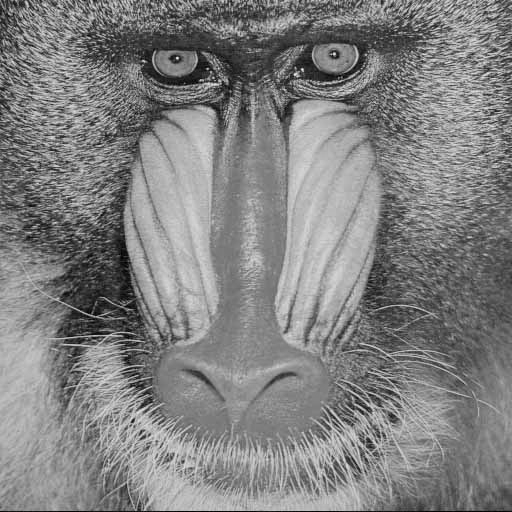
\includegraphics[width=.99\linewidth]{baboon.png}
      \caption{Imagem original (baboon.pgm)}\label{Fig:baboon1}
    \end{minipage}\hfill
    \begin{minipage}{0.48\textwidth}
      \centering
      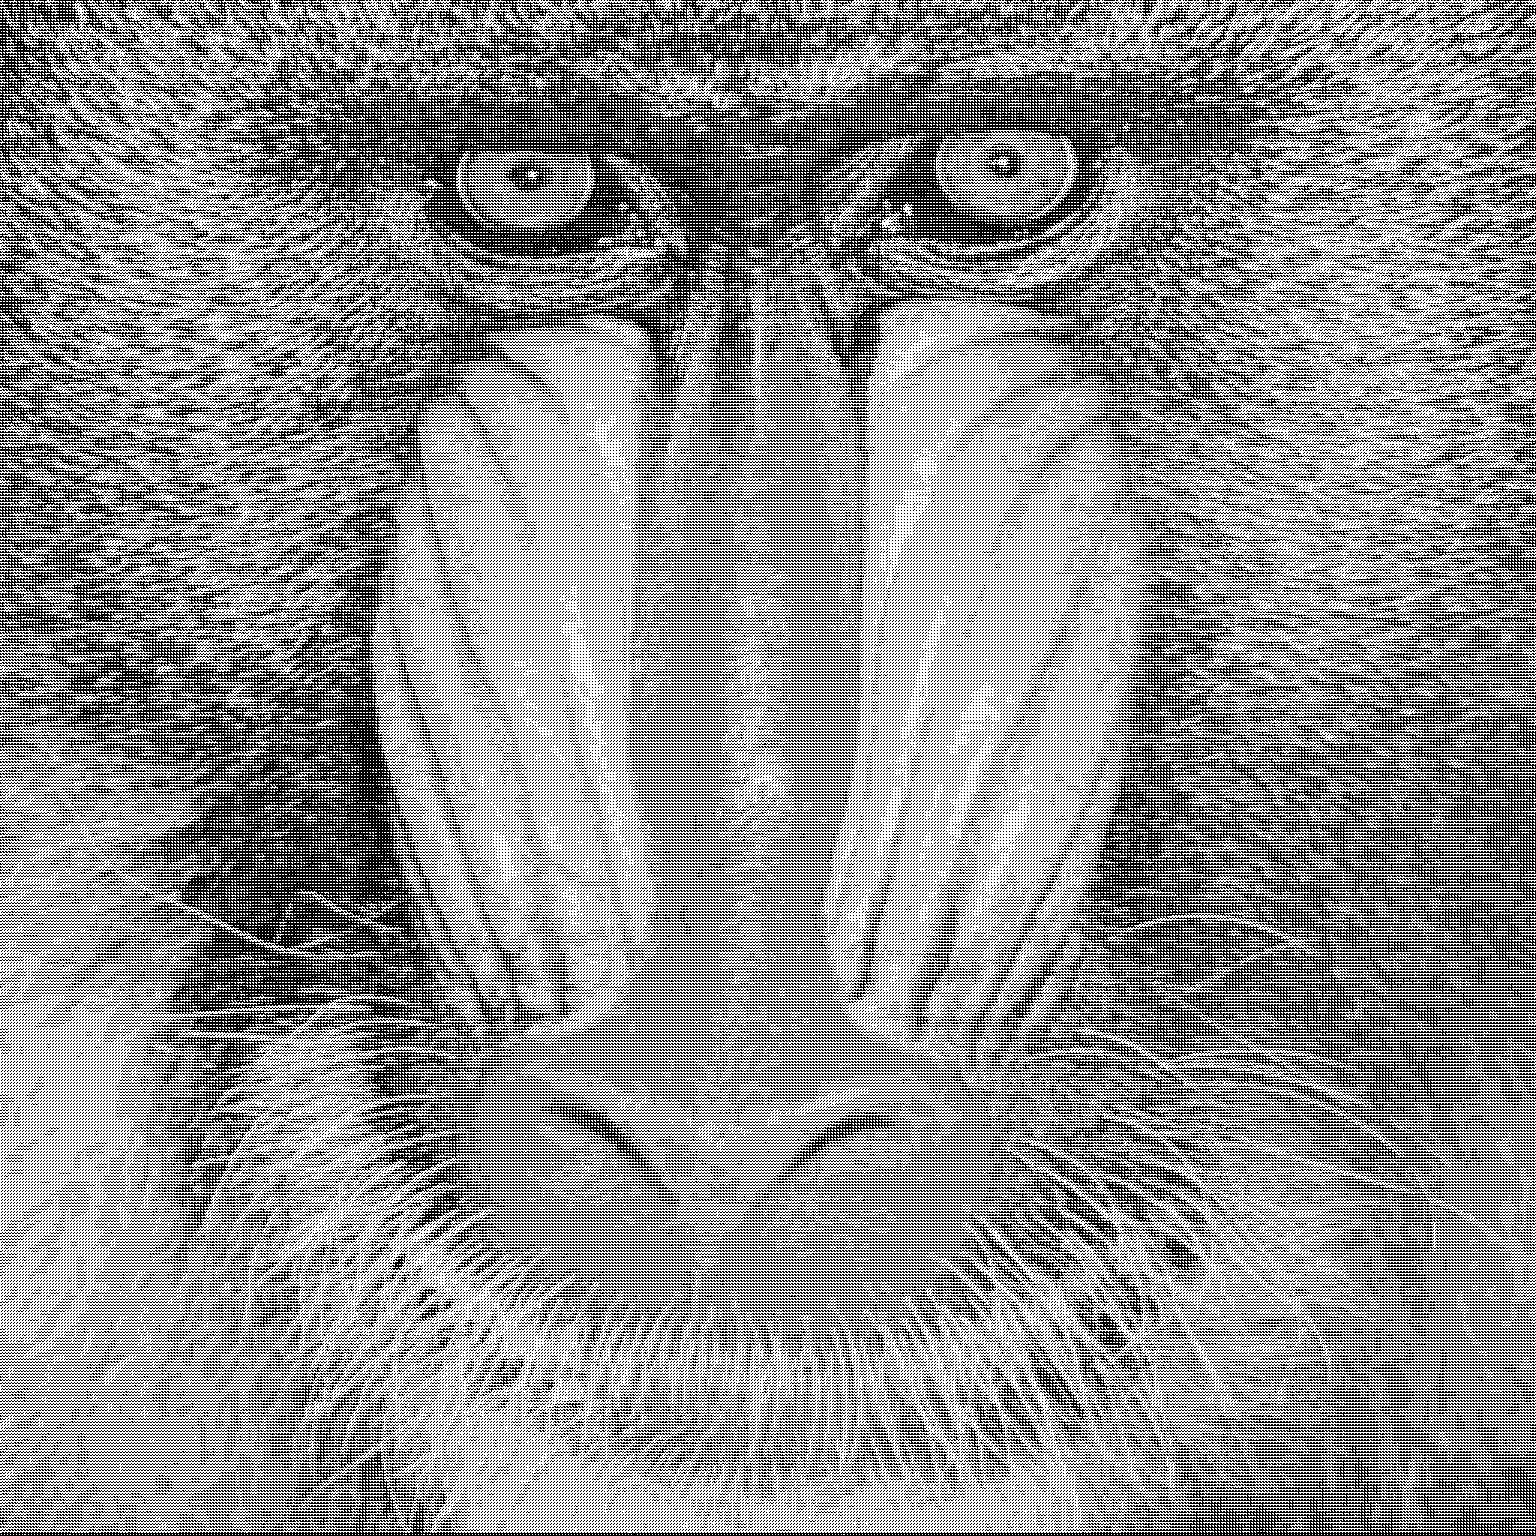
\includegraphics[width=.99\linewidth]{results/image_1.png}
      \caption{Pontilhado ordenado $ M_{3x3}$}\label{Fig:baboon2}
    \end{minipage}
 \end{figure}

\begin{figure}[!htb]
    \begin{minipage}{0.48\textwidth}
      \centering
      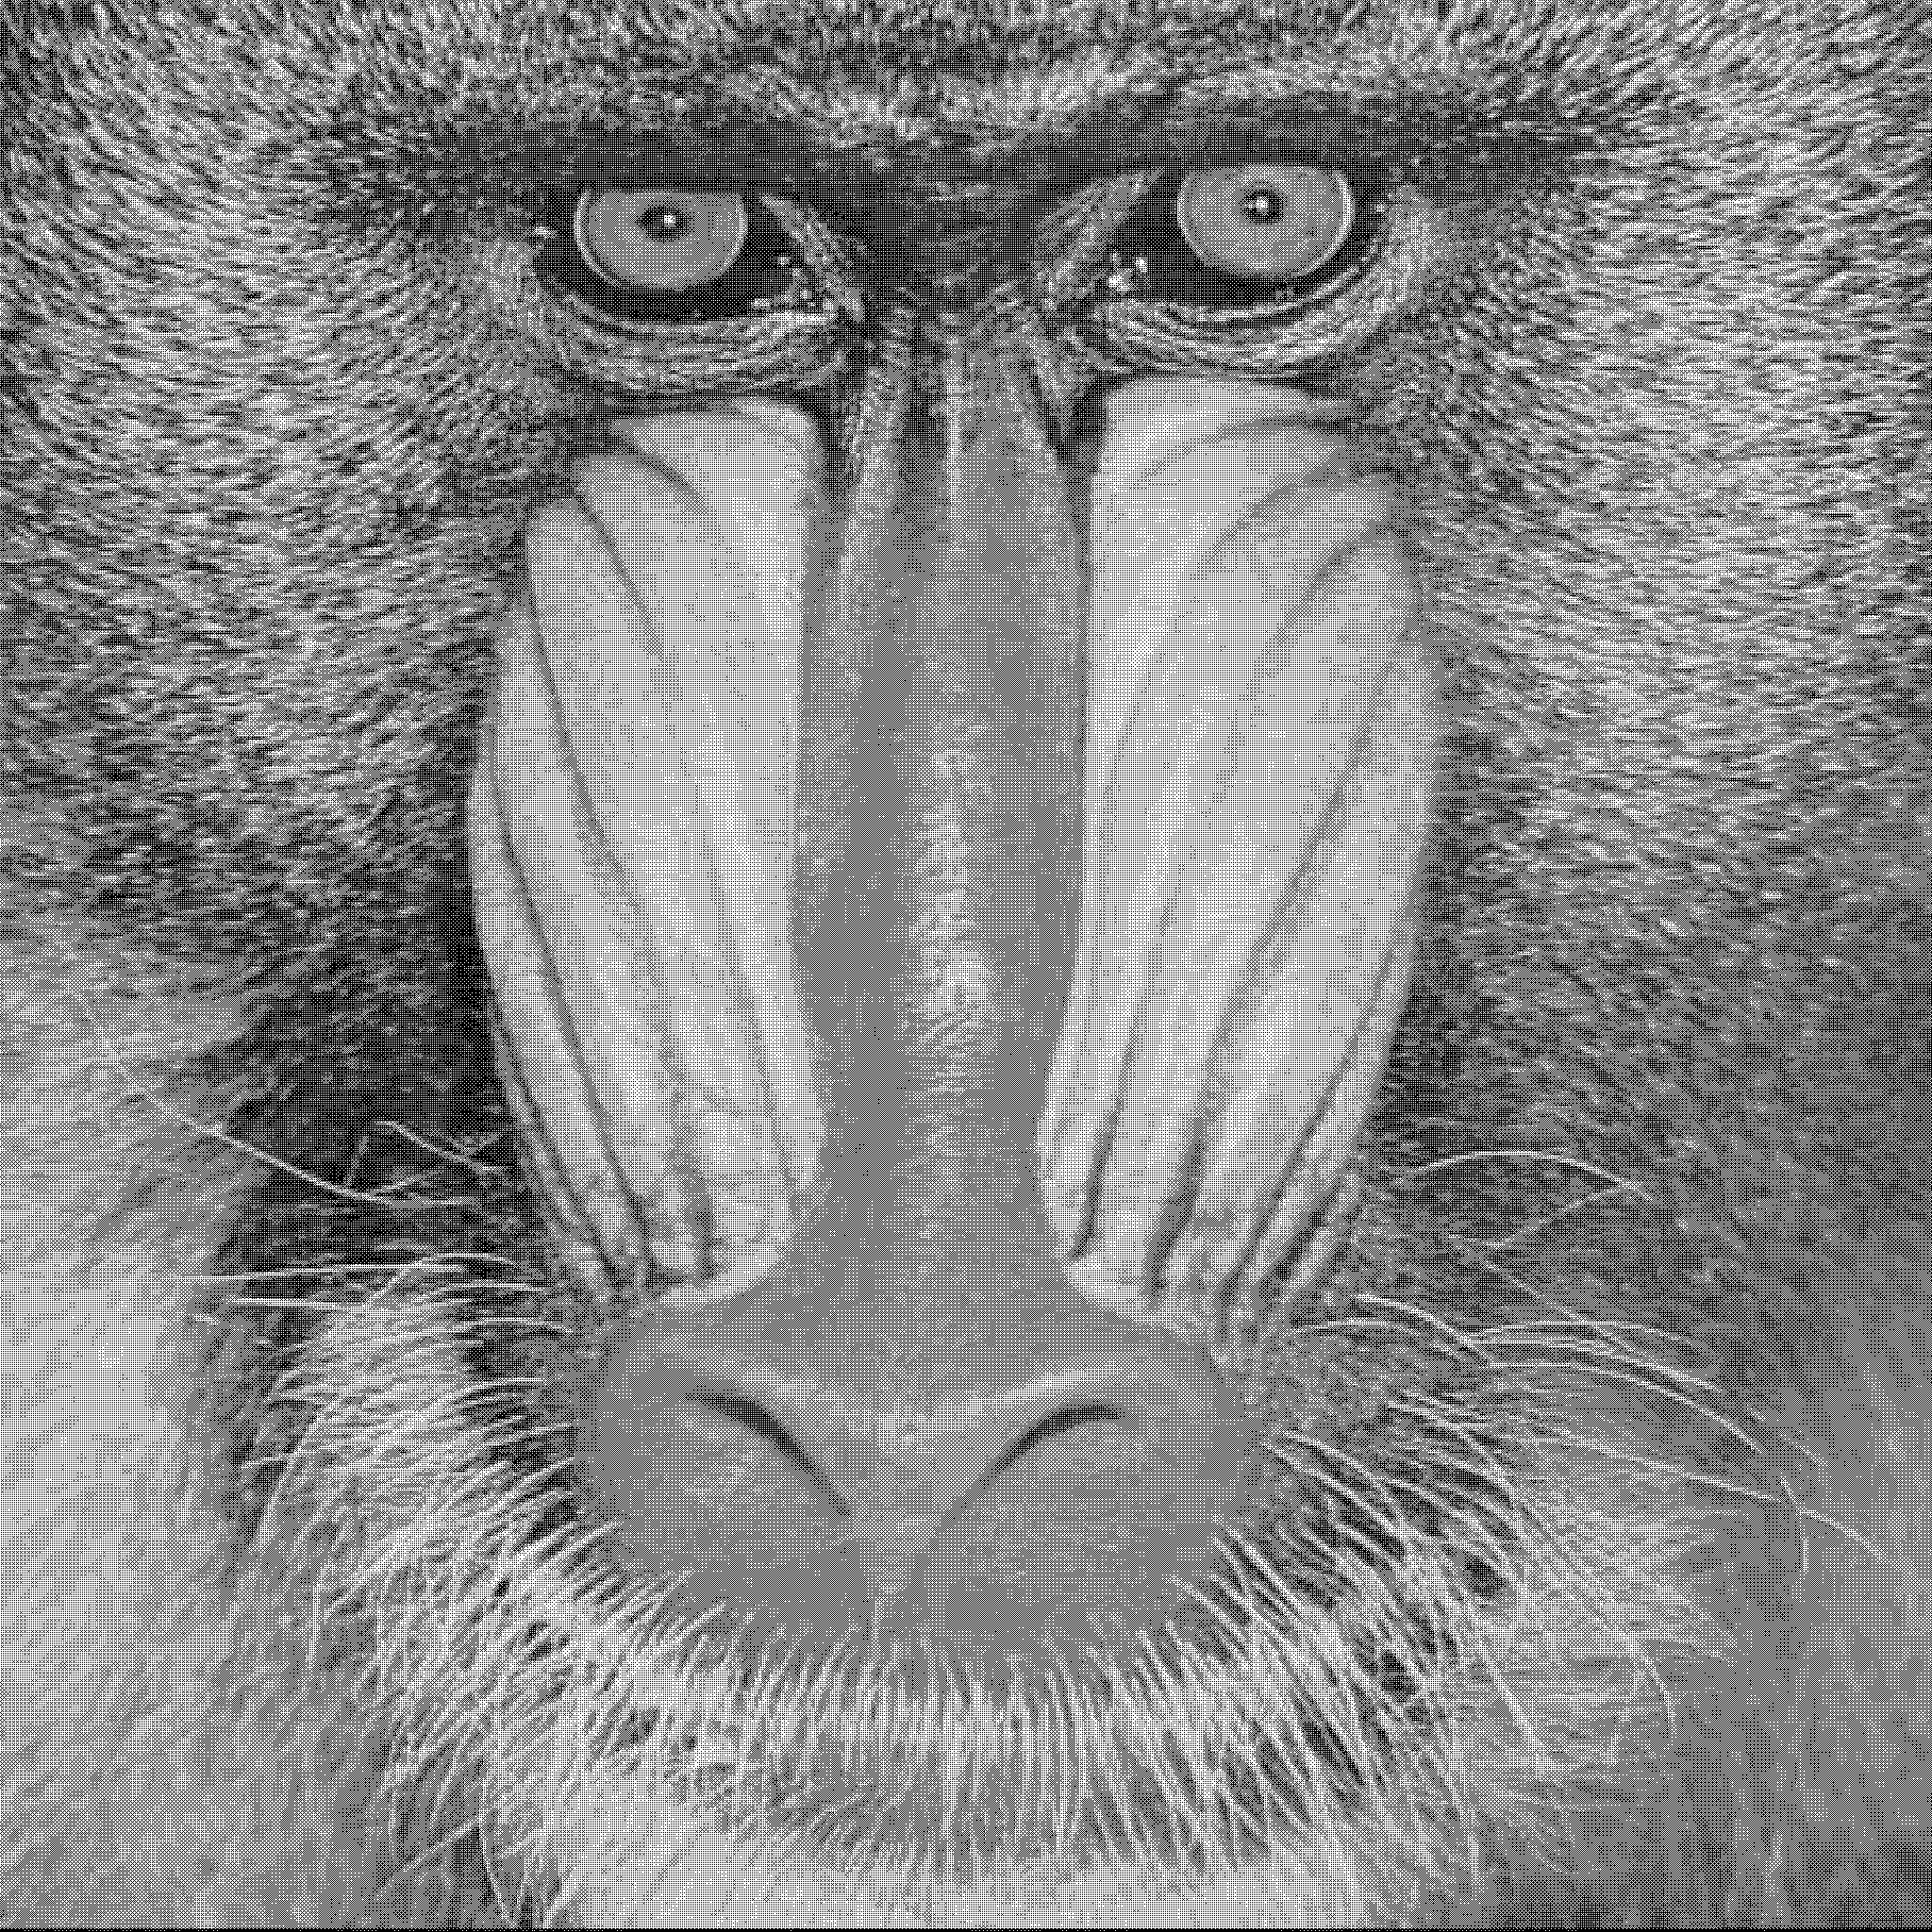
\includegraphics[width=.99\linewidth]{results/image_2.png}
      \caption{Pontilhado ordenado de Bayer}\label{Fig:baboon3}
    \end{minipage}\hfill
    \begin{minipage}{0.48\textwidth}
      \centering
      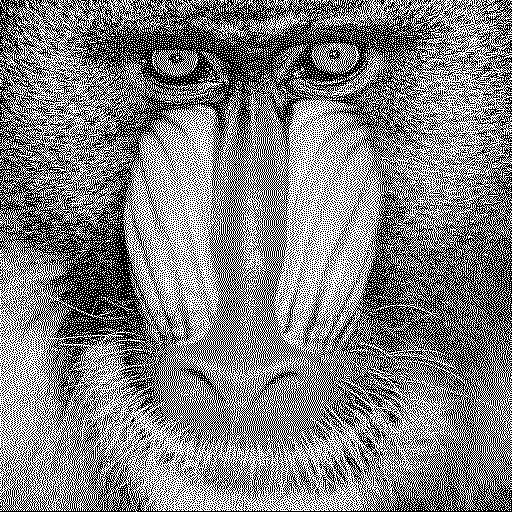
\includegraphics[width=.99\linewidth]{results/image_4.png}
      \caption{Difusão de erro de Floyd-Steinberg}\label{Fig:baboon4}
    \end{minipage}
 \end{figure}


\begin{figure}[!htb]
    \begin{minipage}{0.48\textwidth}
      \centering
      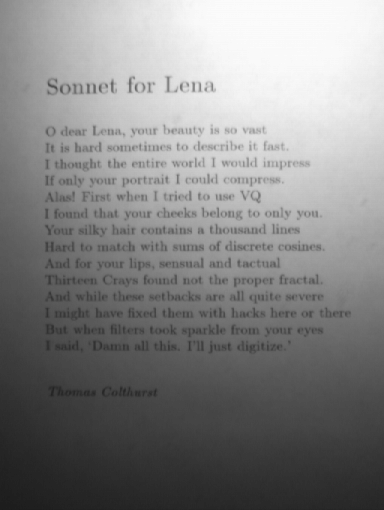
\includegraphics[width=.99\linewidth]{sonnet.png}
      \caption{Imagem original (sonnet.pgm)}\label{Fig:soneto1}
    \end{minipage}\hfill
    \begin{minipage}{0.48\textwidth}
      \centering
      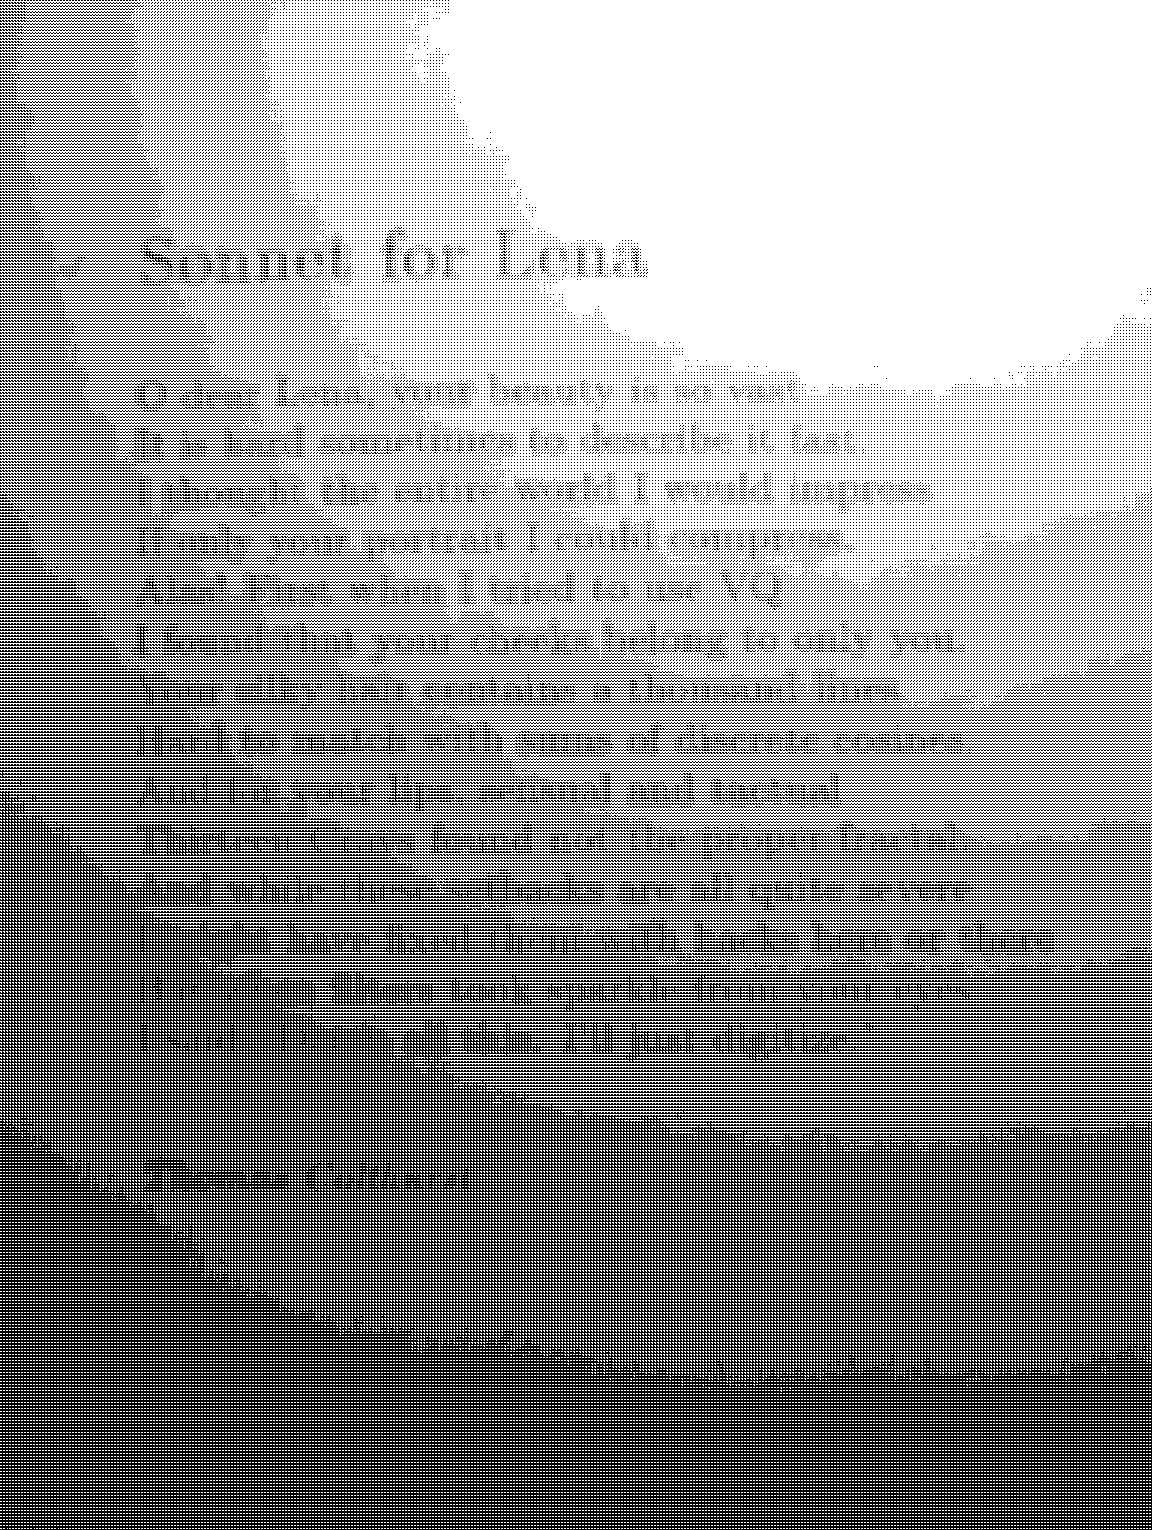
\includegraphics[width=.99\linewidth]{results/image_1_soneto.png}
      \caption{Pontilhado ordenado $ M_{3x3}$ }\label{Fig:soneto2}
    \end{minipage}
 \end{figure}

\begin{figure}[!htb]
    \begin{minipage}{0.48\textwidth}
      \centering
      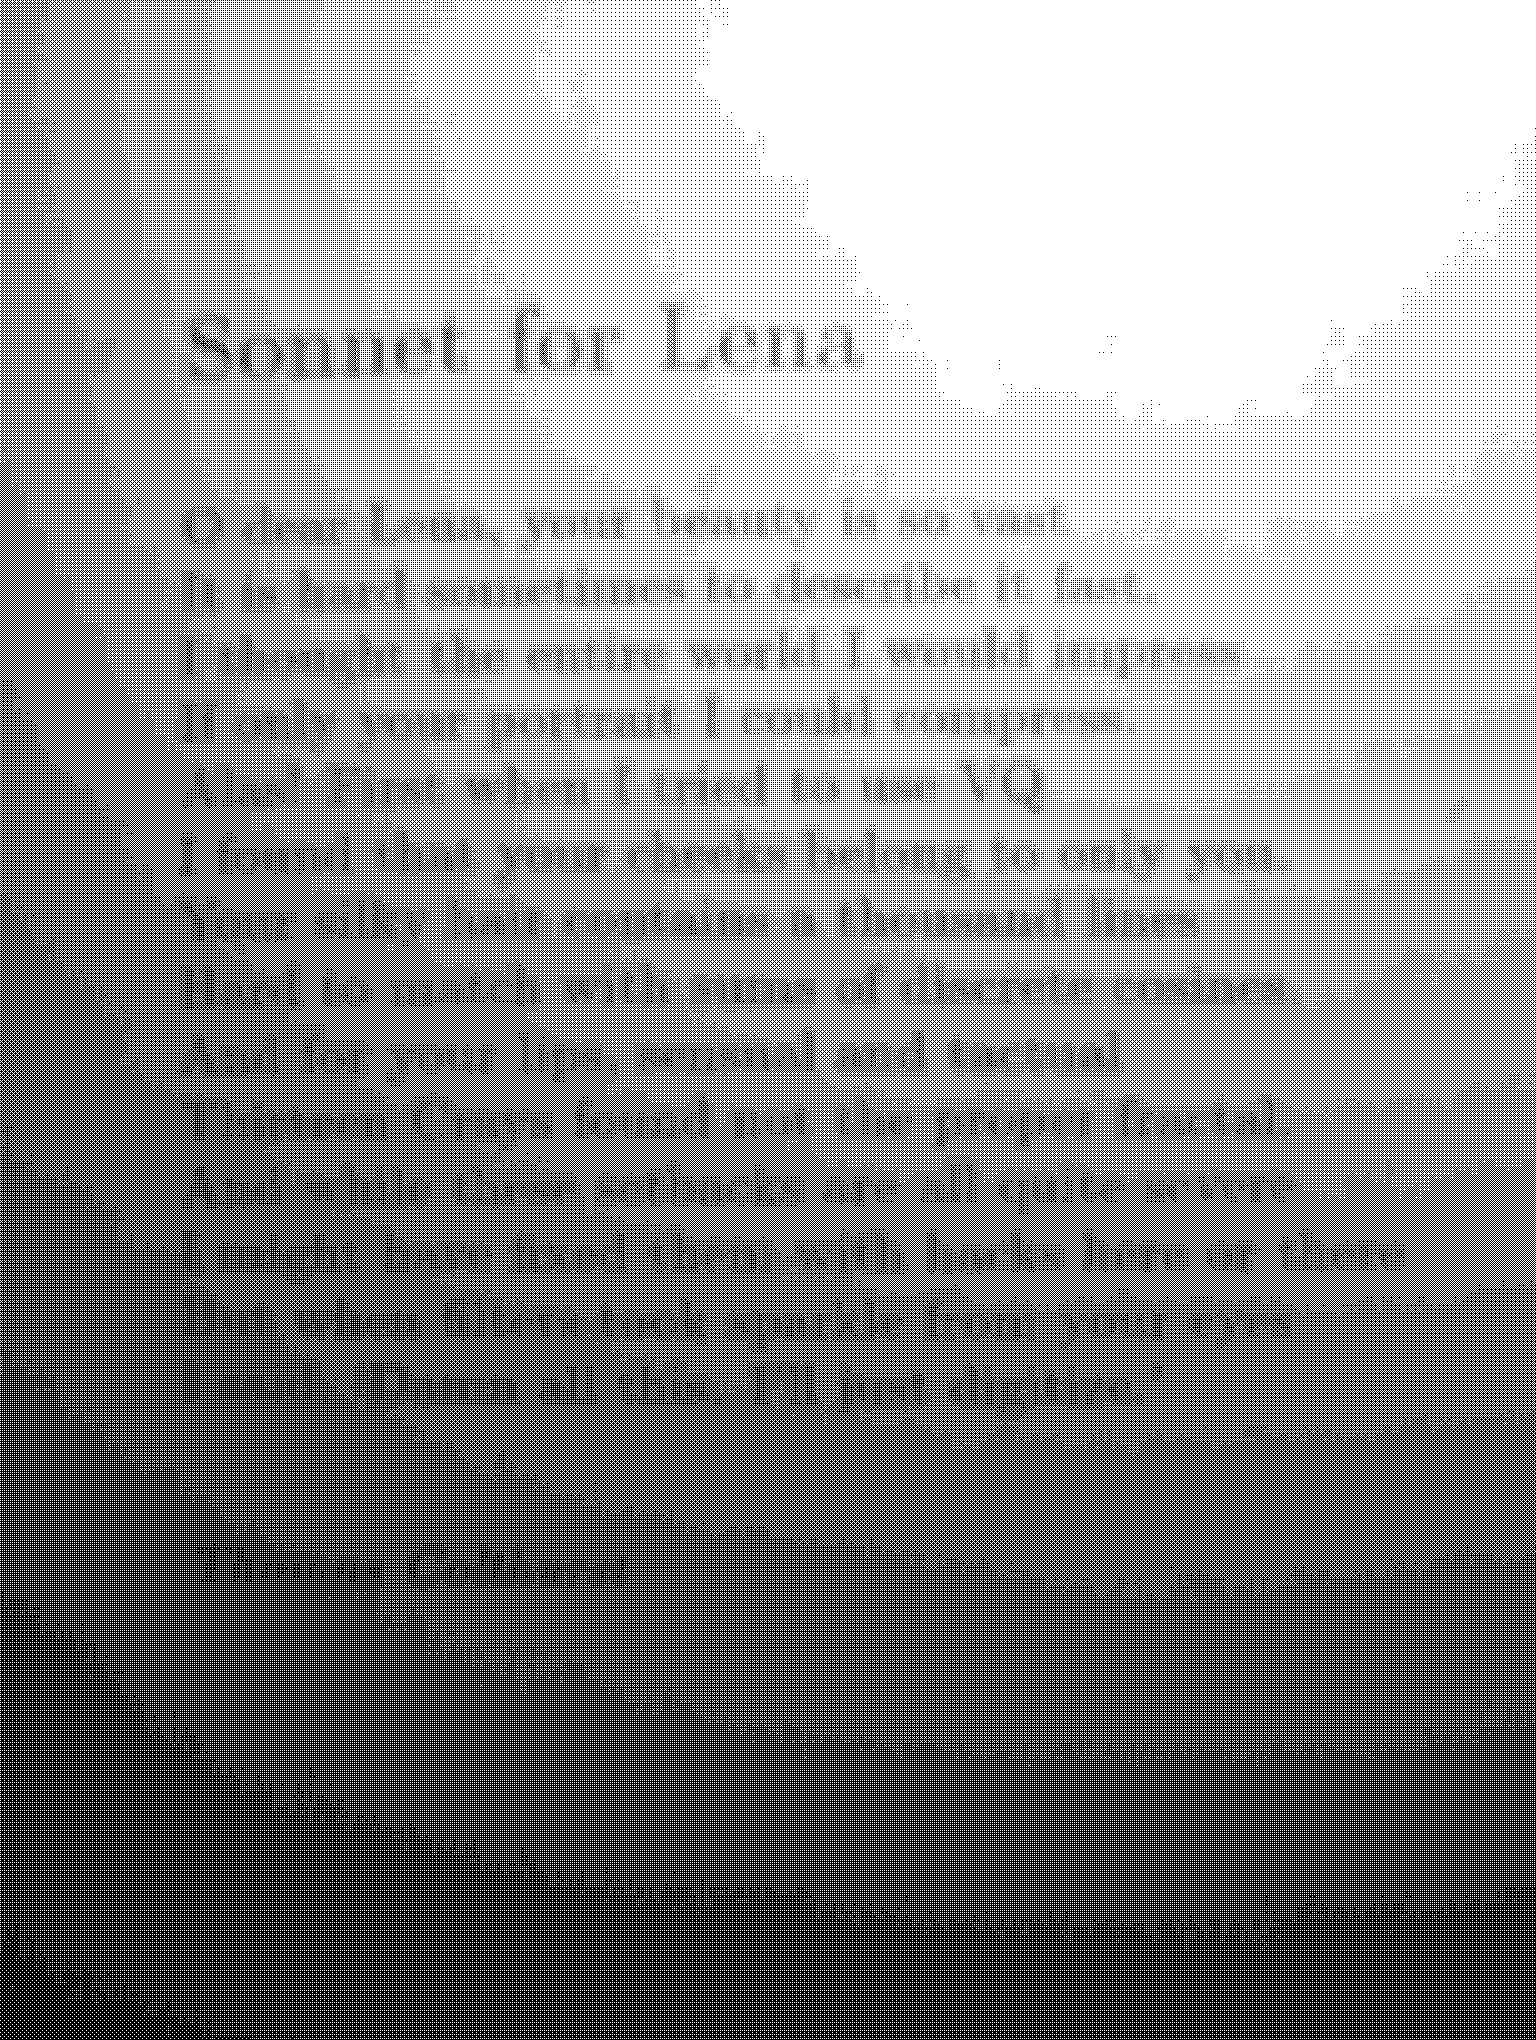
\includegraphics[width=.99\linewidth]{results/image_2_soneto.png}
      \caption{Pontilhado ordenado de Bayer}\label{Fig:soneto3}
    \end{minipage}\hfill
    \begin{minipage}{0.48\textwidth}
      \centering
      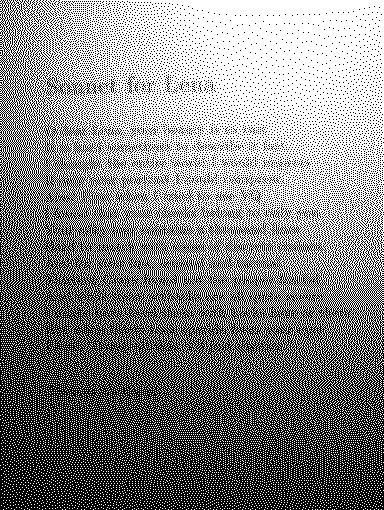
\includegraphics[width=.99\linewidth]{results/image_4_soneto.png}
      \caption{Difusão de erro de Floyd-Steinberg}\label{Fig:soneto4}
    \end{minipage}
 \end{figure}

\bibliography{relatorio2}
\bibliographystyle{ieeetr}

\end{document}